% Source: AESP_466_ClassWork/Supplements/Companion/Euler_Sequences_Quaternions/Euler_Sequences_Quaternions.tex

\documentclass[border=4pt]{standalone}
\usepackage{amsmath}
\usepackage{amssymb}
\usepackage{graphicx}
\usepackage{tikz}
\usepackage{xcolor}
\usetikzlibrary{shapes.geometric, arrows.meta, positioning, decorations.pathmorphing, decorations.pathreplacing, patterns, calc, 3d}

\definecolor{Garnet}{HTML}{73000A}
\definecolor{USC_Rose}{HTML}{CC2E40}
\definecolor{USC_Blue}{HTML}{466A9F}
\definecolor{USC_Slate}{HTML}{1F414D}
\definecolor{USC_Olive}{HTML}{65780B}
\definecolor{USC_Lime}{HTML}{CED318}
\definecolor{USC_Gold}{HTML}{A49137}
\definecolor{USC_Black90}{HTML}{565656}
\definecolor{USC_Black10}{HTML}{ECECEC}

\newcommand{\sectionheader}[1]{%
  \vspace{0.5cm}
  {\noindent\Large \textbf{#1}}
  \vspace{0.2cm}
  \hrule
  \vspace{0.1cm}
  \hrule
  \vspace{0.3cm}
}

\begin{document}
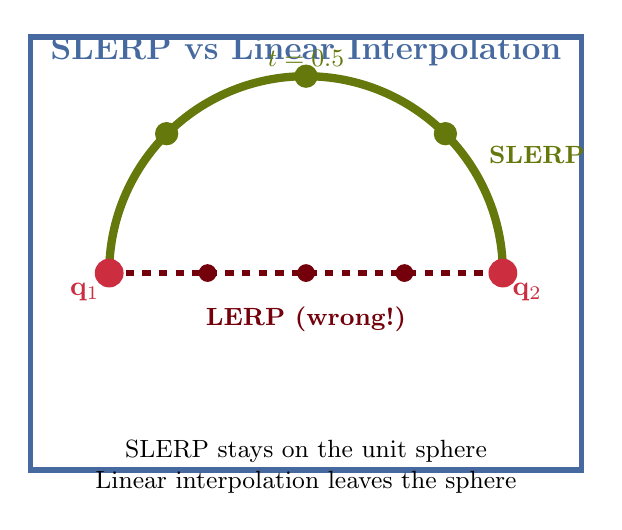
\begin{tikzpicture}[scale=1.0]
    % SLERP visualization
    \draw[draw=USC_Blue, line width=2pt, fill=white] (-3.5,-2.5) rectangle (3.5,3);
    \node[above, USC_Blue, font=\bfseries\large] at (0,2.5) {SLERP vs Linear Interpolation};

    % Arc representing unit sphere great circle (SLERP path)
    \draw[line width=3pt, USC_Olive] (-2.5,0) arc (180:0:2.5);

    % Linear path (chord)
    \draw[line width=2pt, dashed, Garnet] (-2.5,0) -- (2.5,0);

    % Start and end points
    \filldraw[USC_Rose] (-2.5,0) circle (5pt) node[below left, font=\bfseries] {$\mathbf{q}_1$};
    \filldraw[USC_Rose] (2.5,0) circle (5pt) node[below right, font=\bfseries] {$\mathbf{q}_2$};

    % Interpolated points along arc
    \filldraw[USC_Olive] (-1.77,1.77) circle (4pt);
    \filldraw[USC_Olive] (0,2.5) circle (4pt) node[above, font=\small] {$t=0.5$};
    \filldraw[USC_Olive] (1.77,1.77) circle (4pt);

    % Linear interpolated points
    \filldraw[Garnet] (-1.25,0) circle (3pt);
    \filldraw[Garnet] (0,0) circle (3pt);
    \filldraw[Garnet] (1.25,0) circle (3pt);

    % Labels
    \node[USC_Olive, font=\small\bfseries, right] at (2.2,1.5) {SLERP};
    \node[Garnet, font=\small\bfseries, below] at (0,-0.3) {LERP (wrong!)};

    \node[below, font=\small, text width=6cm, align=center] at (0,-2) {SLERP stays on the unit sphere\\Linear interpolation leaves the sphere};
\end{tikzpicture}
\end{document}
